\documentclass{article}
\usepackage{url}
\usepackage{hyperref}
\hypersetup{
    colorlinks=true,
    linkcolor=blue,
    filecolor=magenta,      
    urlcolor=cyan,
}
\usepackage{graphicx}


\newcommand{\BEASTVersion}{2.4.x}
\newcommand{\TracerVersion}{1.6}
\newcommand{\bModelTestVersion}{1.6}

\title{bModelTest in BEAST {\BEASTVersion}\\
Site model averaging without tears}

\author{Remco Bouckaert}

\begin{document}
\maketitle

One of the decisions to make when performing a phylogenetic analysis using nucleotide data is setting up the site model and associated substitution model.
Instead of fixing these settings, bModelTest allows site model averaging through bModelTest \cite{bModelTest}, which makes it easy to set up the site model: just choose bModelTest.
In this tutorial, we go through an analysis using bModelTest in BEAST v\BEASTVersion \cite{beast}, and look into how to interpret the results.
This tutorial assumes you already have done one of the other tutorials, and are familiar with BEAUti, BEAST and Tracer, but if you are not, you may try to start with the Divergence dating tutorial, available from \url{http://beast2.org/tutorials/}.

For this tutorial, you need
\begin{itemize}
\item BEAST version \BEASTVersion, available from \url{http://beast2.org/}
\item Tracer version \TracerVersion, available from \url{http://tree.bio.ed.ac.uk/software/tracer/}
\end{itemize}

We will run through the following steps:
\begin{itemize}
\item{Install bModelTest package}
\item{Set up analysis in BEAUti}
\item{Run analysis with BEAST}
\item{Analyse using Tracer}
\item{Analyse using BModelAnalyser}
\end{itemize}

\section*{Install bModelTest package}
Make sure that you have the bModelTest version \bModelTestVersion package installed. It depends on the BEASTlabs package, which should be installed when you install bModelTest.
See \url{http://beast2.org/managing-packages/} for details on how to install packages.

\section*{Set up analysis in BEAUti}
We will analyse an alignment of 12 primates  with 898 sites \cite{hayasaka1988molecular}. 
\subsection*{Import alignment}First, start BEAUti (restart, if you just installed the bModelTest package through BEAUti), and we need to import the alignment. The alignment is in the file {\tt exampes/neuxs/Primates.nex} which you can find in the BEAST directory. It probably easiest to select the menu {\tt File/Set working dir/BEAST} to start in the BEAST directory, then select menu {\tt File/Import alignment}, and browse to {\tt example/nexus/Primates}.
\subsection*{Link partitions}
After importing the alignment, two partitions will be shown. We want to link everything as if it were a single alignment for this tutorial. To do this, select both alignments in the table, and click the {\tt Link Site Models} button, then {\tt Link Clock Models} and finally {\tt Link Trees}. The screen should look something like this:

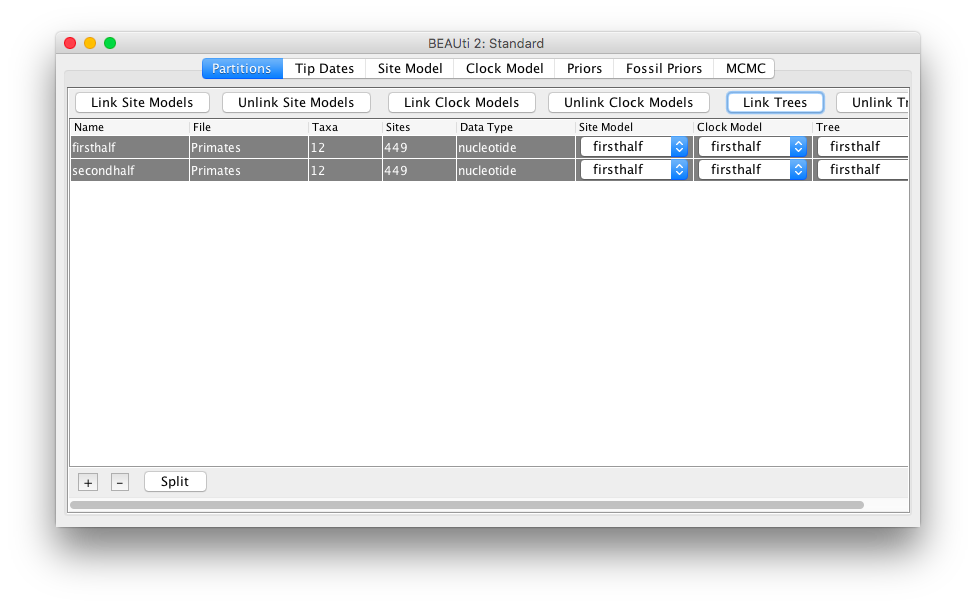
\includegraphics[width=\textwidth]{BEAUti_partitions}
\subsection*{Set up site model}
Click the {\tt Site Model} tab in BEAUti. Select the drop down box at the top which says {\tt Gamma Site Model} and change to {\tt BEAST Model Test}. That's all. The screen should look something like this:

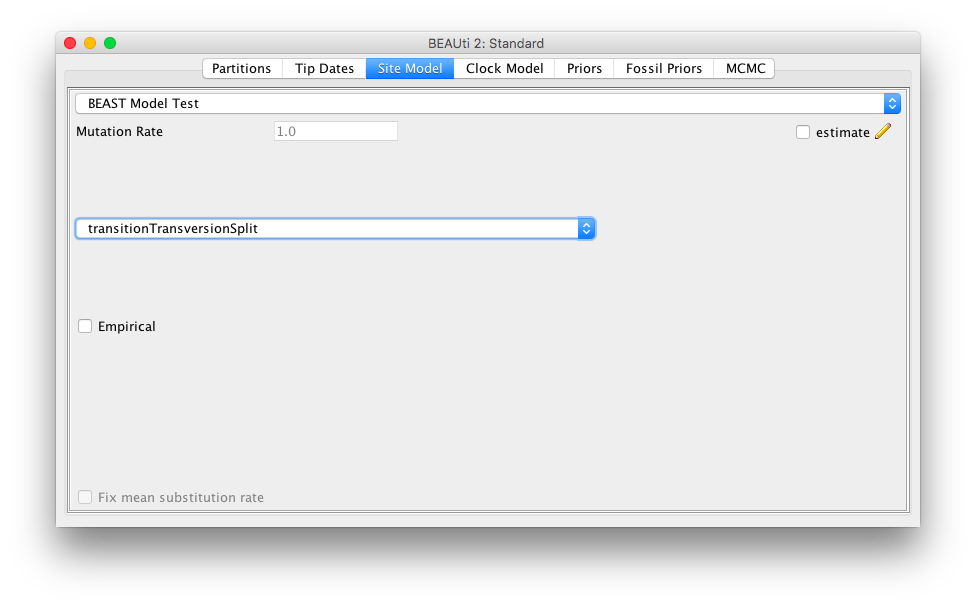
\includegraphics[width=\textwidth]{BEAUti_sitemodel}
\subsection*{Set up clock model}
Click the {\tt Clock model} tab. For this analysis, we use a strict clock, which is the default, so no further changes needed.
\subsection*{Set up priors}
Click the {\tt Priors} tab to show the priors. We will go with default priors for this tutorial.
\subsection*{Set up MCMC}
Click the {\tt MCMC} tab, and change the {\tt chain length} to 2 million, and the file name for the tree trace to {\tt Primates.trees}:

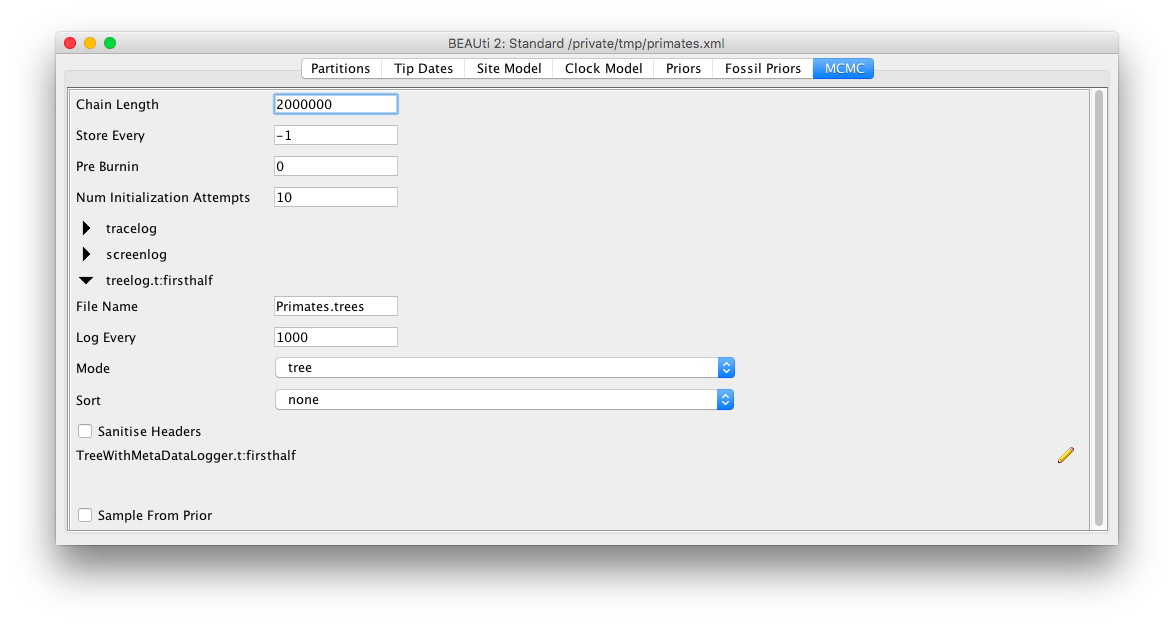
\includegraphics[width=\textwidth]{BEAUti_mcmc}

Save the file using the {\tt File/Save} menu in say {\tt primates.xml}

\section*{Run analysis with BEAST}
Run {\tt primates.xml} using BEAST, as you are used to. Since this is a small alignment, it should take only a minute or two. If ESSs are not satisfactory, you can resume the run for another million samples or so.

\section*{Analyse using Tracer}

Open {\tt Primates.log} in Tracer. You will see the following entries:

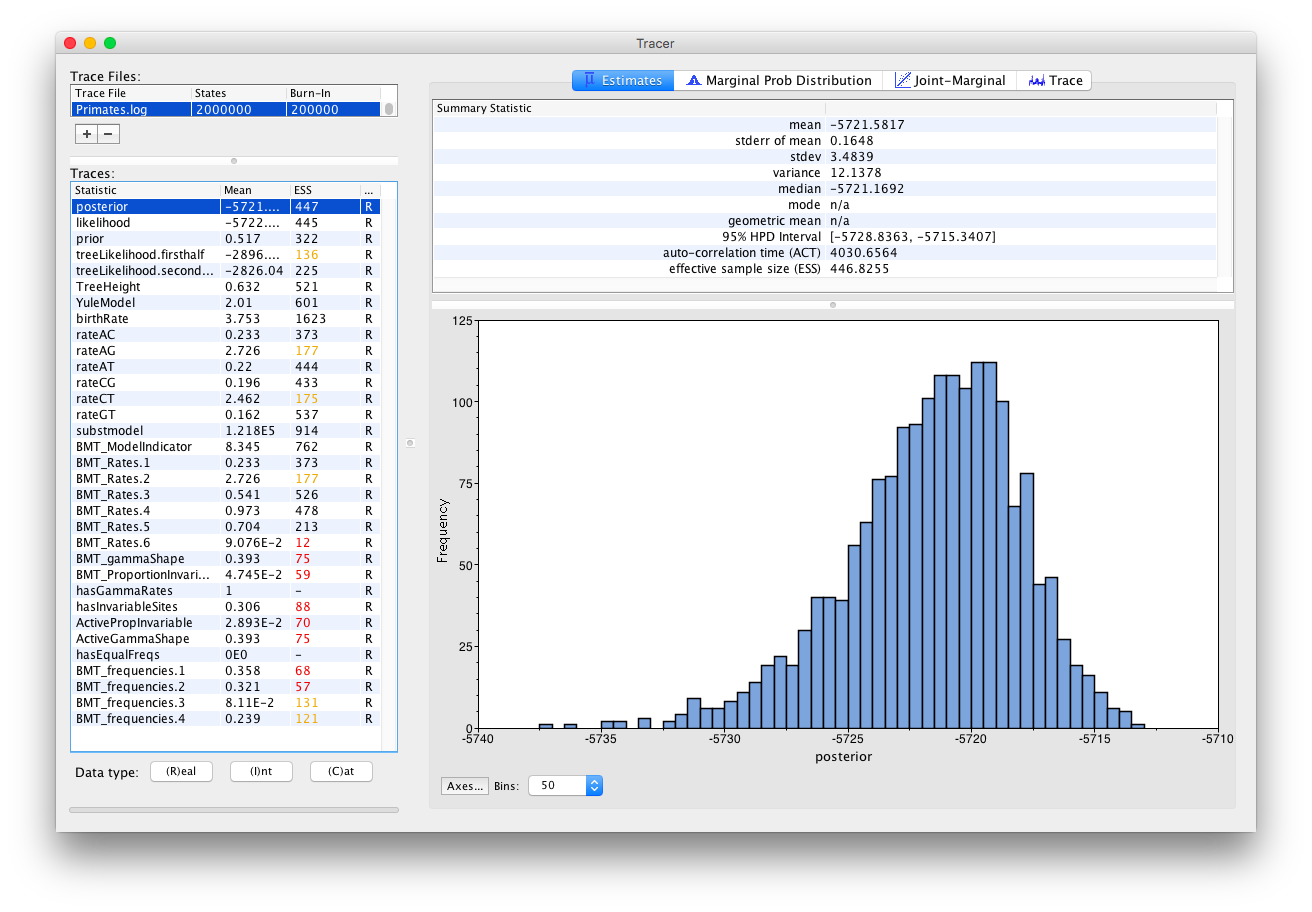
\includegraphics[width=\textwidth]{tracer}

\begin{itemize}
\item BMT\_ModelInidicator is the index of the substitution model as listed in the Appendix.

\item substmodel is the model represented as a 6-digit number, where the position of the digit refers to rates ac, ag, at, cg, ct and gt respectively, and equal digits indicates that rates are shared, so 111111 is Jukes Cantor (if frequencies are kept equal), 121121 is HKY, 123456 is GTR etc.

\item rateAC,\ldots,rateGT are the rates according to the model. ESSs should be good for these rates, but if you plot joint-marginals of pairs you may find high correlation between some of these rates.

\item BMT\_Rates.1 to 6 are the rates used to build up the rate matrix. If only low parameter models are samples, the higher rates will be sampled very infrequently, and you should expect low ESSs for them. Correlation between pairs of rates should be low.

\item BM\_gammaShape is the gamma shape parameter as it is being sampled. For parts of the chain that gamma rate heterogeneity is switched off, the parameter will not be sampled, and the trace will show periods where the parameter is stuck.

\item hasGammaRates indicates whether gamma rate heterogeneity it used (1) or not used (0). The mean can be interpreted as the proportion of time that gamma rate heterogeneity is switched on.

\item ActiveGammaShape is the gamma shape parameter when it is sampled, but it is zero when it it not sampled. To get the estimate of the mean of the shape parameter, divide the mean ActiveGammaShape by the mean of hasGammaRates.

\item BMT\_ProportionInvariable, hasInvariableSites and ActivePropInvariable are the value for proportion invariable similar to BMG\_gammaShape, hasGammaRates and ActiveGammaShape respectively.

\item hasEqualFreqs indicates whether equal frequencies are used and the mean can be interpreted as the proportion of time that equal frequencies is used. When empirical frequencies are used, this parameter is not reported.
\end{itemize}

\section*{Analyse using BModelAnalyser}
BModelAnalyser is a utility that come with the bModelTest package. To start it, in BEAUti select the {\tt File/Launch Apps} menu. A window pops up where you can select the BModelAnalyser App (filter on bModelTest at the top of the dialog if you have many packages).

\begin{center}
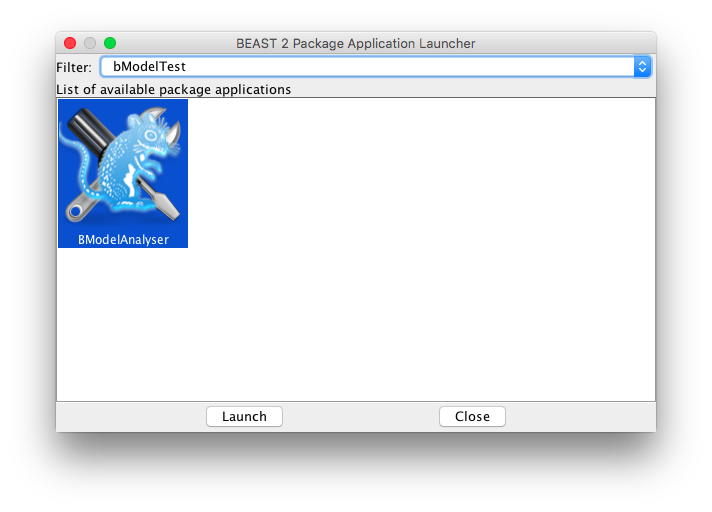
\includegraphics[width=0.6\textwidth]{appstore}
\end{center}

When you click the {\tt Launch} button, after a little while, a dialog appears where you can select the log file:

\begin{center}
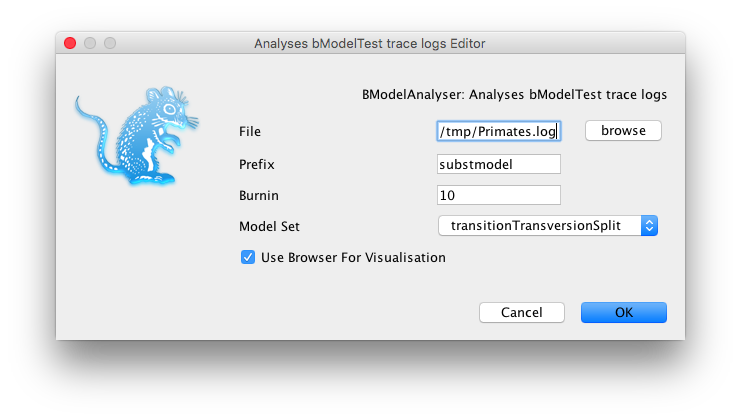
\includegraphics[width=0.7\textwidth]{bModelTestDlg}
\end{center}

\begin{itemize}
\item {\tt File} is the tracelog file produced by BEAST.
\item {\tt Prefix} is the prefix of the entry in the log file containing the substitution model trace (default 'substmodel', which is fine when the analysis is set up in BEAUti)
\item {\tt burnin} is percentage of the log file to disregard as burn-in.
\item {\tt Model Set} is the set of models to choose from, should be the same as used in the BEAST XML that generated the log file, so if you selected a non-default substitution model set, you need to change the model set.
\item {\tt Use Browser For Visualisation} use default web browser for visualising the resulting dot graph.
\end{itemize}
Click OK, and a console pops up with model coverage results.

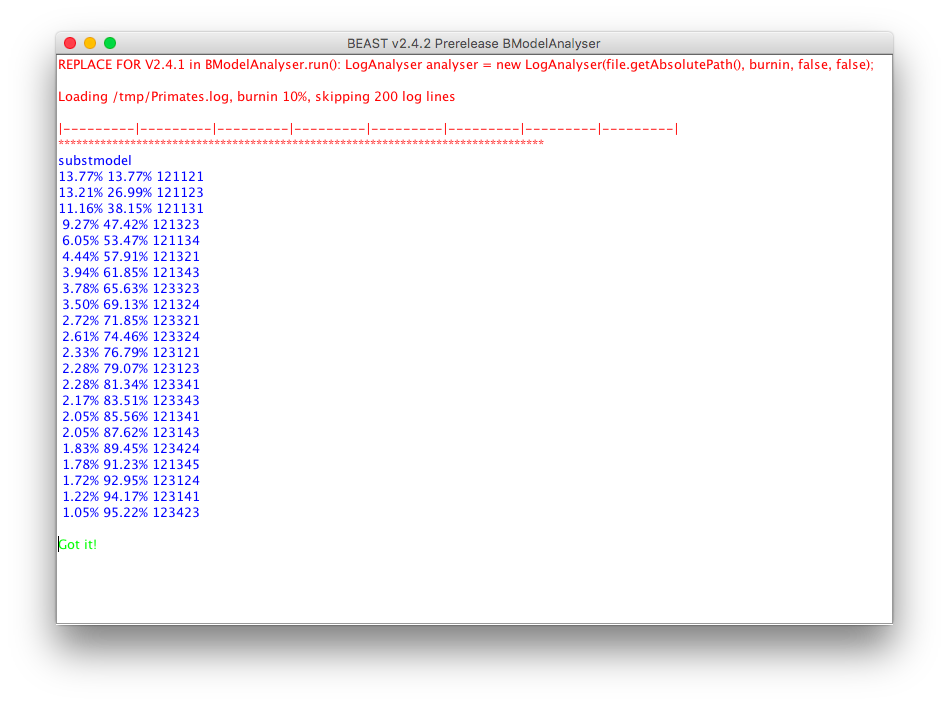
\includegraphics[width=\textwidth]{bModelTest0}

After a little while, a page is opened in your web browser containing the same information, but better formatted, and it shows a graph containing the models, which should look something like this:

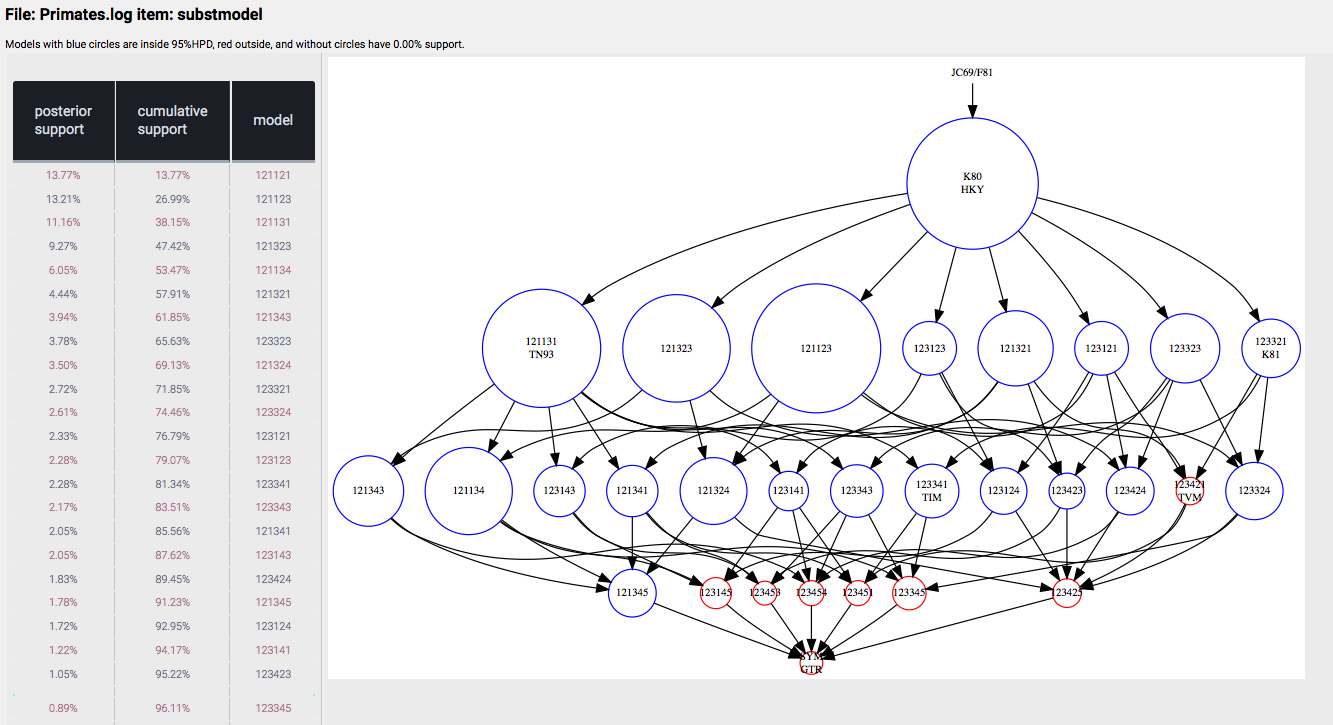
\includegraphics[width=\textwidth]{bModelTest}

Arrows indicate that the model at the tail is nested inside the model at the head and can be obtained by adding one parameter to the model.

The area of the circles around models are proportional to the posterior support for these models. In this case, we see a lot of support for HKY, 121123 and TN93.

Blue circles indicate the model is contained in the 95\% credible set, red circles indicate the model is outside the 95\% credible set, and no circles indicate there is hardly any support (if at all) in the posterior.

If you would like to reproduce the graph with dotty, a {\tt .dot} file is generated called {\tt[pacakge dir]/2.4/bModelTest/js/bModelTest0.dot} where {\tt [pacakge dir]} depends on your operating system: 
{\tt \textasciitilde/Library/Application Support/BEAST} for OSX, {\tt C:\textbackslash Users\textbackslash}{\tt[your name]\textbackslash BEAST} on Windows and {\tt \textasciitilde/.beast} on Linux.

\bibliographystyle{plain}
\bibliography{bModelTestTutorial}

\end{document}
